%%%%%%%%%%%%%% 
% Fichero: EjTablas
% Autor: J. Salido (http://www.uclm.es/profesorado/jsalido)
% Fecha: febrero, 2017
% Descripción: Ejemplo básico de inclusión de tablas.
% Ejemplo del curso: “LaTeX esencial para preparación de TFG, Tesis
% y otros documentos académicos” (Esc. Sup. Informática-UCLM)
%%%%%%%%%%%%%%




%%%%%%%%%%%%%%
% Preámbulo del documento
%%%%%%%%%%%%%%
\documentclass[11pt,a4paper]{article} 
\usepackage[utf8]{inputenx} 
\usepackage[spanish, es-tabla]{babel} 
\usepackage[left=2cm,right=2cm,top=2cm,bottom=2cm]{geometry} % Márgenes 

% Tipografía
\usepackage{newpxtext}
\usepackage{newpxmath}

\usepackage{marvosym}
\usepackage{pifont} % Generación de símbolos especiales
\usepackage{textcomp}

\usepackage[T1]{fontenc} % Codificación de salida    
\usepackage{microtype} % Mejoras de microtipografía en la obtención de PDF (sólo para pdflatex)

\usepackage{url} % Para escritura de URL
\urlstyle{sf}

% Generación de hiperenlaces
\usepackage[pdftex,breaklinks,colorlinks,
			citecolor=blue, % Color de la citas
			urlcolor=blue, % Color de las URL
			bookmarksnumbered=true, % Incluye números en bookmarks
			pdftitle={Fundamentos de LaTeX para principiantes},
			pdfauthor={Jesús Salido},
			pdfsubject={LaTeX}]{hyperref}

% Listas
\usepackage{paralist} % Mayor control de listas
\usepackage{multicol} % Elementos en varias columnas


% Gráficos
\usepackage{graphicx}  % Inclusión de figuras y escalado de cajas

% Declaración del path donde están los archivos de figuras. 
% También se puede incluir el path en el nombre del fichero.
\graphicspath{{../figs/}}  
\DeclareGraphicsExtensions{.pdf,.png,.jpg}
% Lista de extensiones de ficheros por orden de precedencia. De este modo no hace falta indicar la extensión del fichero y en caso de existir dos fichero con el mismos nombre y extensión diferente se emplea el que tiene una extensión con mayor prioridad.


\usepackage[margin=10pt,labelfont=bf]{caption} % Configuración de caption en objetos float
\captionsetup[table]{skip=5pt} 	% Separación del caption en las tablas aumentando el valor por defecto 


% Con estas instrucciones se ajustan los valores del índice
\setcounter{secnumdepth}{1} % Ajusta el valor del último nivel numerado
\setcounter{tocdepth}{2} %Ajusta el valor del último nivel que aparece en TOC



\author{Jesús Salido}
\title{Inclusión de tablas básicas en \LaTeX{}}
\date{\today}


%%%%%%%%%%%%%%
% Comienzo del documento
%%%%%%%%%%%%%%
\begin{document}

\maketitle


\begin{abstract}
	Explicación sencilla sobre cómo incluir y manejar las tablas con \LaTeX{}.
\end{abstract}

\tableofcontents


\listoftables





\section{Tablas en \LaTeX{}}
La inclusión de tablas en documentos preparados con \LaTeX{} no es sencilla e incluso podría calificarse de <<engorro>>. Las tablas se crean con el entorno \texttt{tabular} en el que se indica el número de columnas y la alineación del texto en cada columna (l=izda., c=central, r=dcha.). Las líneas de separación en la tabla se indican mediante el caracter \texttt{`|'} (líneas verticales) o la macro \texttt{\textbackslash hline} (líneas horizontales). La separación del texto entre columnas se realiza con el caracter \texttt{`\&'} y la separación de filas con \texttt{`\textbackslash\textbackslash'}. Para que la tabla sea manejada como un objeto \emph{float} debe incluirse en el entorno \texttt{table}.

Estos conceptos se muestra en el siguiente ejemplo:

% Ejemplo
% ==========
\begin{table}[hbt]%
	\centering
	\caption[Ejemplo de entorno \texttt{table}]{Los grupos de alimentos}		  \label{tab:alimentos}
	\begin{tabular}{| l | c | r | }
		\hline			
		\textbf{Cítricos} & \textbf{Legumbres} & \textbf{Hortalizas} \\ \hline \hline
		Naranja  & Judía     & Tomate \\ \hline
		Limón    & Garbanzo  & Pepino \\ \hline  
	\end{tabular}
\end{table}

En el ejemplo de la tabla~\ref{tab:alimentos} se muestra una tabla con un conjunto importante de propiedades como: líneas de separación (horizontales y verticales), distintos tipos de justificación, etc. Como puede comprobarse en dicho ejemplo, \LaTeX{} es capaz de realizar las tablas con multitud de elementos con una gran flexibilidad. Sin embargo, echando un vistazo al texto fuente podemos intuir que la elaboración de tablas es tediosa y tanto más cuanto mayor sea el tamaño y la complejidad de la tabla.

En el siguiente ejemplo se ha hecho uso de la macro \texttt{cline} para generar líneas que no abarcan todas las columnas de la tabla.

% Ejemplo
% ==========
\begin{table}[hbt]%
	\centering
	\caption{Ejemplo de uso de la macro \texttt{cline}}
	\label{tab:cline}
	\begin{tabular}[t]{|r|l|}
	\hline
	7C0 & hexadecimal \\[1cm] % Ejemplo de separación fijada entre líneas
	3700 & octal \\ \cline{2-2}
	11111000000 & binario \\
	\hline \hline
	1984 & decimal \\
	\hline
	\end{tabular}
\end{table}

Hay que tener cuidado con la longitud del contenido de cada celda ya que, por defecto, \LaTeX{} no recorta el texto al tamaño de la línea. Para evitarlo se especifica el ancho de columna:

% Ejemplo
% ==========
\begin{table}[hbt]%
	\centering
	\caption{Ejemplo de tabla con especificación de anchura de columna}
	\label{tab:anchura}
	\begin{tabular}{ | l | l | l | p{5cm} |}
	\hline
	Día & Temp Mín (\textdegree C) & Temp Máx (\textdegree C) & Previsión \\ \hline
	Lunes & 11 & 22 & Día claro y muy soleado. Sin embargo, la brisa de la tarde puede hacer que las temperaturas desciendan \\ \hline
	Martes & 9 & 19 & Nuboso con chubascos en muchas regiones. En Cataluña claro con posibilidad de bancos nubosos al norte de la región \\ \hline
	Miércoles & 10 & 21 & La lluvía continuará por la mañana pero las condiciones climáticas mejorarán considerablemente por la tarde\\
	\hline
	\end{tabular}
\end{table}

Cuando las tablas tienen muchas columnas es posible hacer una declaración abreviada empleando la sintaxis \texttt{*\{num\}\{just\}} como en la tabla siguiente:

% Ejemplo
% ==========
\begin{table}[hbt]%
	\centering
	\caption{Especificación abreviada en tabla}
	\label{tab:abreviada}
	\begin{tabular}{l*{6}{c}|r}
	Equipo            & J & G & P & E & F  & C & Pts \\
	\hline
	Manchester United & 6 & 4 & 0 & 2 & 10 & 5 & 12  \\
	Celtic            & 6 & 3 & 0 & 3 &  8 & 9 &  9  \\
	Benfica           & 6 & 2 & 1 & 3 &  7 & 8 &  7  \\
	FC Copenhagen     & 6 & 2 & 1 & 2 &  5 & 8 &  7  \\
	\end{tabular}
\end{table}

Cuando se emplean tablas con datos numéricos a veces puede interesar la alineación de datos por el signo de puntación empleado para la separación de decimales (\texttt{`,'} en español, \texttt{`.'} en inglés). Un ejemplo de esto se ilustra a continuación:

% Ejemplo
% ==========
\begin{table}[hbt]%
	\centering
	\caption{Tabla numérica con alineación al caracter `,'}
	\label{tab:alineada}
	\begin{tabular}{c r@{,} l}
	Expresión con pi & \multicolumn{2}{c}{Valor} \\
	\hline
	$\pi$                   &      3 & 14159 \\
	$\pi^{\pi}$             & 36     &    46 \\
	$(\pi^{\pi})^{\pi}$     &  80662 & 7     \\
	\end{tabular}
\end{table}


\newpage
\section{Tablas incluidas como figuras}
Tal como muestran los ejemplos precedentes la preparación de tablas con \LaTeX{} es un proceso de cierta complejidad. Por el contrario las tablas, confeccionadas mediante hojas de cálculo, que puede incluirse en los documentos con los procesadores tipo WYSIWYG (Word, OpenOffice, etc.) siguen un proceso intuitivo y rápido. Existe un modo para aprovechar estas ventajas empleando \LaTeX{}. Para ello se puede salvar en formato PDF las tablas creadas con una hoja de cálculo (p.ej.\ \textsf{Excel}) e incorporarlas en un documento \LaTeX{} mediante una tabla que sólo contiene una celda en la que incluimos el fichero gráfico con la tabla en formato PDF. En la tabla~\ref{tab:figura} se muestra un ejemplo de una tabla creada con \textsf{Excel}. Este método permite emplear las tipografías disponibles en el sistema para las hojas de cálculo. Además se puede aplicar todas las opciones aplicables para los gráficos incluido el dimensionado de los mismos. Es importante señalar que si no se va a aplicar ningún escalado a la figura de la tabla, ésta debería crearse con el mismo tamaño de fuente que tendrá el texto normal del documento final y empleando preferiblemente una tipografías lo más similar posible a la utilizada en el documento.

% Ejemplo:
% ============
\begin{table}[hbt]%
	\centering
	\caption[Tabla \textsf{Excel}]{Ejemplo de tabla creada con \textsf{Excel} e incluida como figura}
	\label{tab:figura}
	\begin{tabular}{c}
		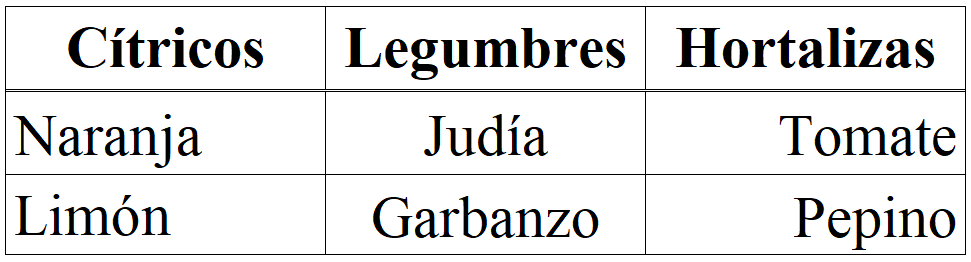
\includegraphics{alimentos}
	\end{tabular}
\end{table}

Este método es aceptable para publicaciones como TFG y Tesis. Sin embargo, no es apropiado para publicaciones especializadas (p.~ej.\ revistas y congresos) y en estos casos la editorial suele rechazar el resultado por los estándares tan exigentes empleados. El problema deriva de que las fuentes empleadas por los programas externos emplean tipografías ligeramente diferentes a las empleadas por \LaTeX.


\end{document}
